\subsection{Objetivo 3 --- generalização para \On{N}}

\textit{Propor e implementar a generalização do Oracle em diferentes níveis.}

Implementada para todo $N=1,\dots,M$, com a curva completa gravada por fold. A
relação de monotonicidade $\On{1}\ge\On{2}\ge\dots\ge\On{M}$ --- que é a definição da
medida, não uma hipótese --- foi verificada em \textbf{$1450/1450$ folds, sem
exceção}.

\begin{table}[htbp]
\centering\small
\caption{Níveis de Oracle e métodos reais, média sobre $29$ bases $\times$ $10$ folds.}
\begin{tabular}{lrrrrrrr}
\toprule
Modo & \On{1} & \On{2} & \On{5} & \On{M} & \mvr & Comb.\ suave & Acc.\ indiv. \\
\midrule
PGDCS completo  & 0.9972 & 0.9953 & 0.9897 & 0.1139 & 0.7771 & 0.7752 & 0.7042 \\
PGDCS-F1/T1     & 0.9976 & 0.9963 & 0.9905 & 0.1179 & 0.7784 & 0.7738 & 0.7052 \\
Bags aleatórios & \textbf{0.9979} & 0.9957 & 0.9901 & 0.1158 & 0.7808 & 0.7768 & 0.7046 \\
Bagging         & 0.9951 & 0.9935 & 0.9884 & \textbf{0.3052} & 0.8467 & 0.8466 & 0.7931 \\
Random Forest   & 0.9970 & \textbf{0.9958} & \textbf{0.9920} & 0.1725 & \textbf{0.8549} & 0.8546 & 0.7806 \\
\bottomrule
\end{tabular}
\end{table}

A tabela já antecipa o problema central do objetivo 7: entre $N=1$ e $N=5$ a curva
cai apenas de $0.997$ para $0.990$, enquanto a votação majoritária está em
$0.78$--$0.85$. A faixa conservadora que o subprojeto procurava não está aqui.

\begin{figure}[htbp]
\centering
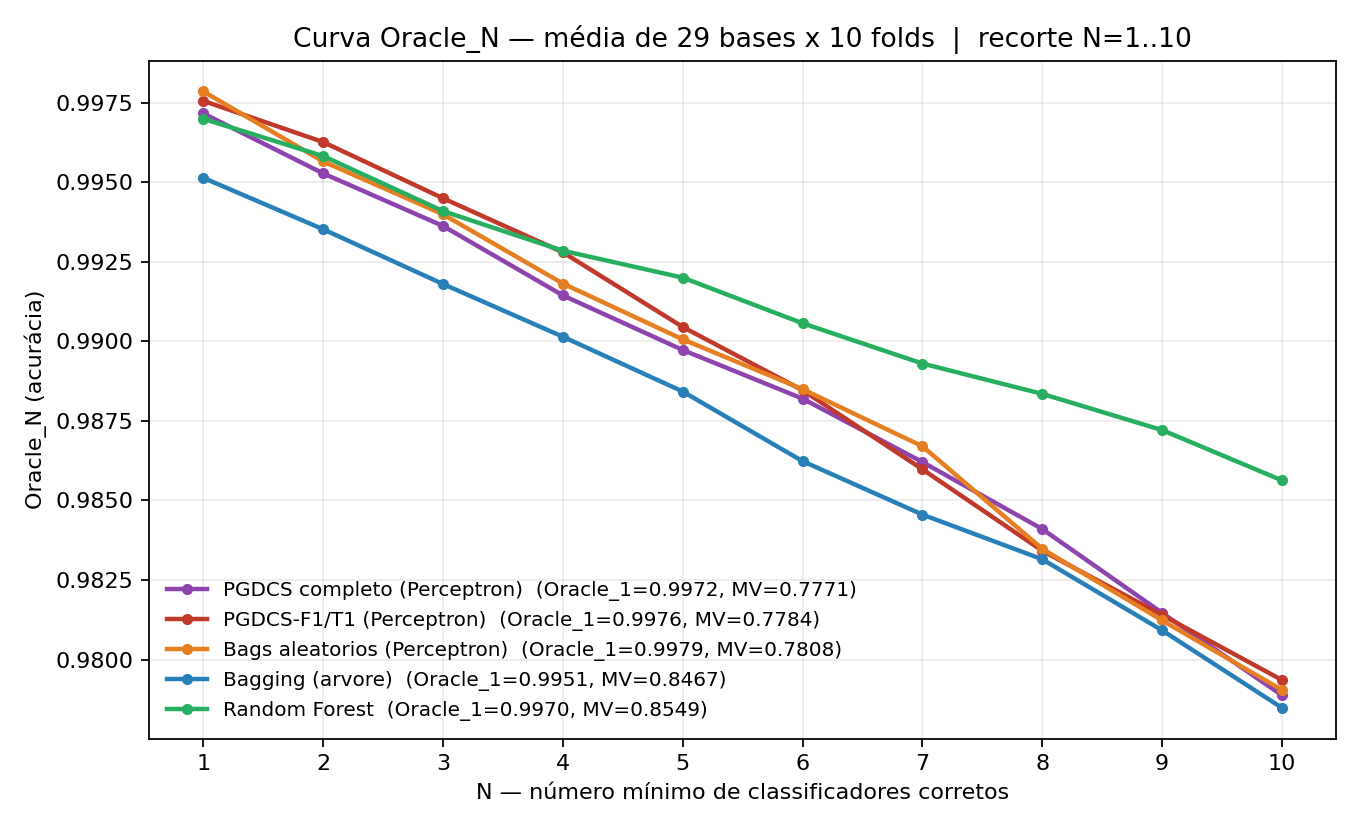
\includegraphics[width=0.86\textwidth]{figuras/fig2_oracle_curve_zoom.png}
\caption{Curva \On{N} no recorte $N=1..10$, com a votação majoritária de cada modo.
A distância vertical entre a curva e a linha tracejada correspondente é a folga.
Os três pools de Perceptron lideram em $N=1$, mas o Random Forest os ultrapassa a
partir de $N=3$: a vantagem do pool de menor acurácia individual existe só na ponta
mais otimista, e a Seção 5 mostra que ela não distingue entre os três métodos de
geração --- só entre classificadores-base.}
\end{figure}
